\subsection{Draw}

$draw(f,x)$ draws a graph of function $f$ of $x$.
(The default second argument is $x$.)

{\color{blue}
\begin{verbatim}
draw(x^2)
\end{verbatim}
}

\begin{center}
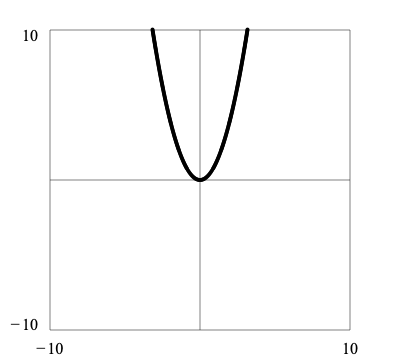
\includegraphics[scale=0.5]{parabola1.png}
\end{center}

\noindent
The vectors $xrange$ and $yrange$ control the scale of the graph.

{\color{blue}
\begin{verbatim}
xrange = (-1,1)
yrange = (0,2)
draw(x^2)
\end{verbatim}
}

\begin{center}
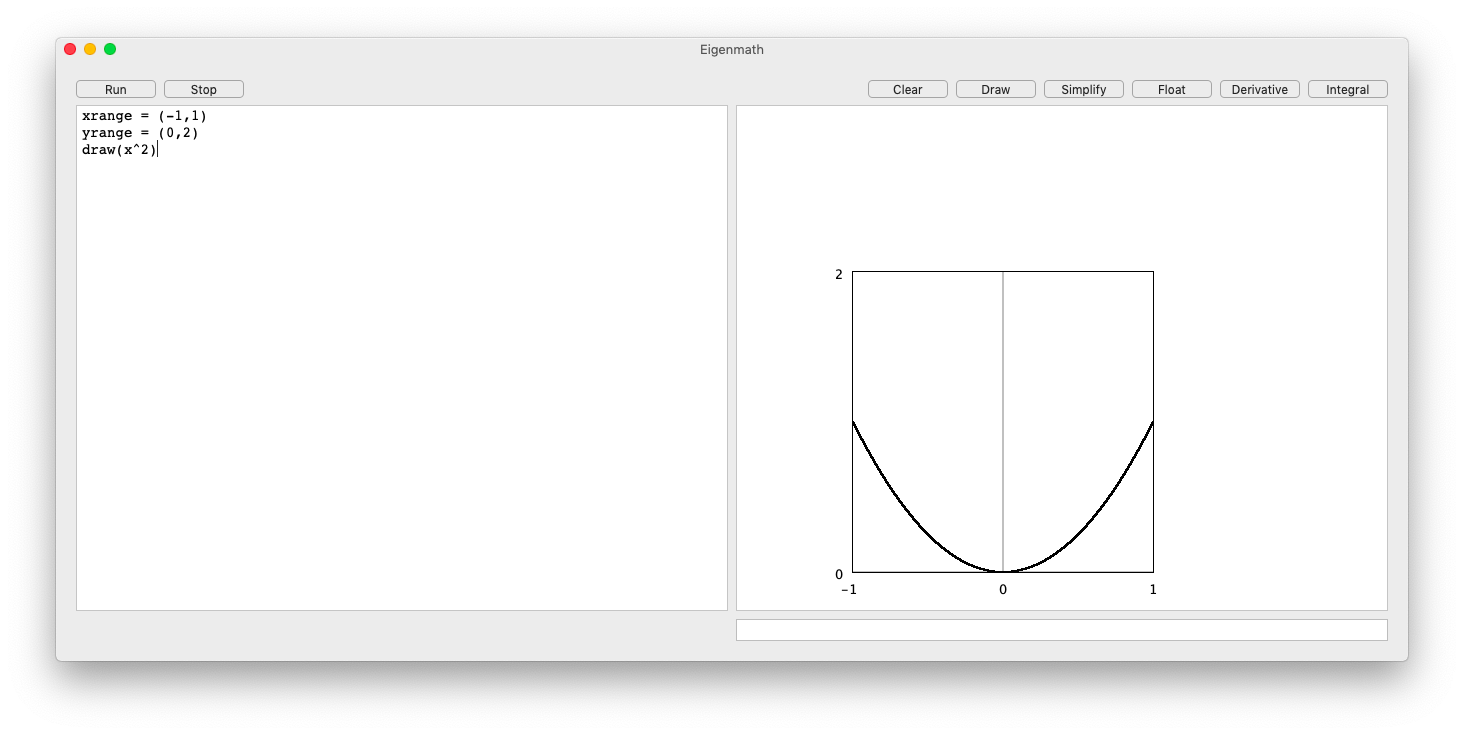
\includegraphics[scale=0.5]{parabola2.png}
\end{center}

\noindent
Parametric drawing occurs when a function returns a vector.
The vector $trange$ controls the parametric range.
The default is $trange=(-\pi,\pi)$.
In the following example, $draw$ varies $theta$
over the default range $-\pi$ to $+\pi$.

{\color{blue}
\begin{verbatim}
xrange = (-10,10)
yrange = (-10,10)
f = 5 (cos(theta),sin(theta))
draw(f,theta)
\end{verbatim}
}

\begin{center}
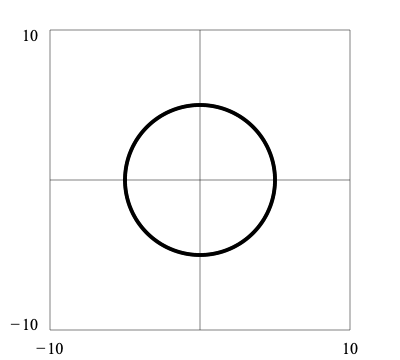
\includegraphics[scale=0.5]{circle1.png}
\end{center}

\noindent
In the following example, $trange$ is reduced
to draw a quarter circle instead of a full circle.

{\color{blue}
\begin{verbatim}
trange = (0,pi/2)
f = 5 (cos(theta),sin(theta))
draw(f,theta)
\end{verbatim}
}

\begin{center}
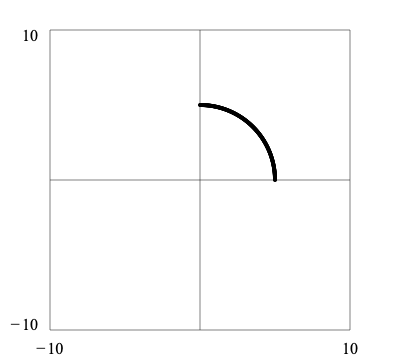
\includegraphics[scale=0.5]{circle2.png}
\end{center}

\noindent
Lemniscate.

{\color{blue}
\begin{verbatim}
trange = (-pi,pi)
X = cos(t) / (1 + sin(t)^2)
Y = sin(t) cos(t) / (1 + sin(t)^2)
f = 5 (X,Y)
draw(f,t)
\end{verbatim}
}

\begin{center}
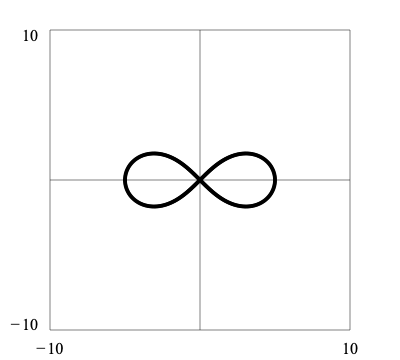
\includegraphics[scale=0.5]{lemniscate.png}
\end{center}

\noindent
Cardioid.

{\color{blue}
\begin{verbatim}
r = (1 + cos(t)) / 2
u = (cos(t),sin(t))
f = r u
xrange = (-1,1)
yrange = (-1,1)
trange = (0,2pi)
draw(f,t)
\end{verbatim}
}

\begin{center}
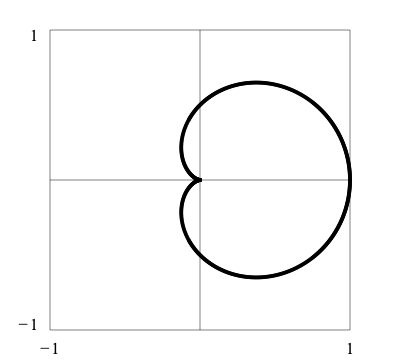
\includegraphics[scale=0.5]{cardioid.png}
\end{center}
